\section{Durchführung}
\label{sec:Durchführung}

\begin{figure}[H]
    \centering
    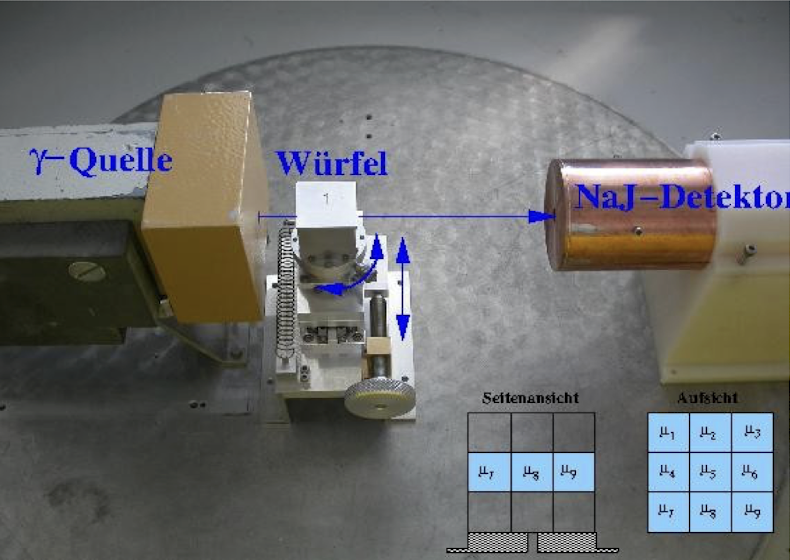
\includegraphics[scale=0.8]{Abbildungen/Aufbau.pdf}
    \caption{Schematischer Aufbau des Versuchs.\cite{V46}}
    \label{fig:aufbau}
\end{figure}

Der Aufbau des Versuchs ist in \autoref{fig:aufbau} dargestellt.
Als Lichtquelle wird eine Halogen-Lampe verwendet, welche ein überwiegend infrarotes Emissionsspektrum liefert, da der verwendete Halbleiter
GaAs durchlässig für infrarotes Licht ist.
Die Strahlung fällt zunächst durch eine Linse um möglichst parallele Lichtstrahlen zu erzeugen.
Ein Lichtzerhacker in Form einer sich drehenden Sektorscheibe befindet sich als nächstes im Strahlengang um das Licht in Impulse zu zerlegen.
Danach trifft das Licht auf ein Glan-Thompson-Prisma, dessen Aufgabe es ist, das Licht linear zu polarisieren.
Die Funktionsweise eines Glan-Thompson-Prismas ist schematisch in \autoref{fig:prisma} dargestellt. Die Polarisationsebenen der beiden
austretenden Strahlen stehen orthogonal aufeinander.
\begin{figure}[H]
    \centering
    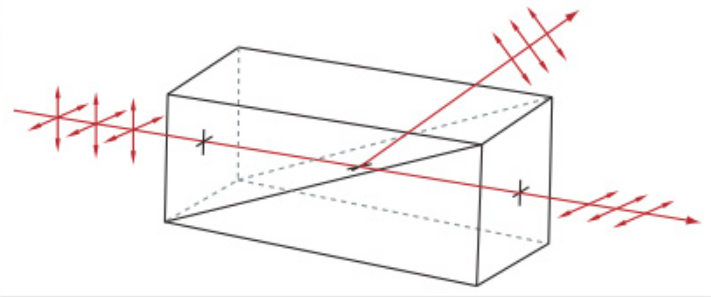
\includegraphics[scale=0.35]{Abbildungen/prisma.png}
    \caption{Strahlengang in einem Glan-Thompson-Prisma.\cite{Prisma}}
    \label{fig:prisma}
\end{figure}
Am Prisma befindet sich zudem ein Goniometer zur Winkelmessung.
Das Licht tritt dann durch den Spalt zwischen den Elektromagneten und durch die Probe, die sich in einem Luftspalt in den Elektromagneten
befindet.
Der Wellenvektor des Lichtfeldes ist hierbei parallel zum zeitlich konstanten Magnetfeldvektor, der durch die Elektromagneten erzeugt wird.
Die Elektromagneten sind an einen Polwender angeschlossen, der dafür sorgt, dass keine gefährlichen Induktionsspannungen beim Umpolen enststehen.
Nach den Elektromagneten passiert das Licht einen Interferenzfilter, wo eine bestimmte Wellenlänge des Lichts herausgefiltert wird.
Das Licht ist nun monochromatisch und wird in einem weiteren Glan-Thompson-Prisma in
zwei zueinander senkrecht polarisierte Komponenten zerlegt.
Mithilfe von Sammellinsen werden die beiden Strahlen nun auf Photowiederstände gelenkt, welche die Intensität messen.
Die entstehenden Signale gelangen nun an einen Differenzverstärker, dessen Ausgangsspannung proportional zur Differenz der beiden Eingangsspannungen
ist und somit verschwindet, wenn beide Eingangsspannungen in Betrag und Phase übereinstimmen.
Der darauf folgende Selektivverstärker wird auf die durch den Lichtzerhacker erzeugte
Modulationsfrequenz abgestimmt, sodass Störfrequenzen bestmöglich herausgefiltert werden.
Zur Darstellung der Signalamplitude ist dem Selektivverstärker ein Oszilloskop nachgeschaltet.

\subsection{Justage des Versuchsaufbaus}
\label{sub:Justage}

Die Apparatur wird vor der eigentlichen Messung justiert. Dafür werden zunächst die Probe und der Interferenzfilter aus dem Strahlengang
entfernt. Zur Justage wird sichtbares Licht verwendet.
Im nächsten Schritt wird die Polarisationsvorrichtung überprüft. Die Prismen sollten so gedreht werden, dass das Licht senkrecht auf ihre Oberfläche fällt.
Außerdem wird überprüft ob das Licht auf den Sensitivbereich der jeweiligen Photodioden fällt und gegebenenfalls angepasst.
fallen. Das Licht soll so auf die Detektoren treffen, dass bei geeigneter Drehung des Polarisationsprimsas die Lichtintensität an einem der Detektoren verschwindet und beim anderen maximal wird.
Der Lichtzerhacker wird in Bewegung gesetzt und eine Frequenz von $\qty{450}{\hertz}$ eingestellt.
Die Verstärkerfrequenz des Selektivverstärkers wird nun so variiert, dass die Signalamplitude am Oszilloskop maximal wird.




\subsection{Messung zur Bestimmung der Magnetfeldstärke}
\label{sub:Magnetfeld}

Im ersten Teil der Messung wird die Kraftflussdichte $B(x)$ mittels einer Hall-Sonde gemessen.
Der Feldstrom wird hierfür auf einen Maximalwert geregelt. Mit der Sonde wird dann für verschiedene Abstände $x$ der zugehörige
Wert des Magnetfelds bestimmt. Es soll besonders der Bereich des Luftspaltes, wo eigentlich die Probe steht, untersucht werden.


\subsection{Messung zur Bestimmung der Drehwinkel}
\label{sub:Drehwinkel}

Für die eigentliche Messung wird eine Probe und ein Interferenzfilter in den Aufbau eingesetzt. Bei eingeschaltetem Magnetfeld wird das erste Glan-Thompson-Prisma
so gedreht, dass die auf dem Oszilloskop angezeigte Signalamplitude minimal wird und am Goniometer wird der Winkel $\theta_1$ abgelesen.
Nun wird das Feld umgepolt, wieder ein Nullabgleich durchgeführt und der Winkel $\theta_2$ am Goniometer abgelesen.
Mit diesem Verfahren werden jeweils zwei Winkel pro Interferenzfilter aufgenommen. Die Messung wird für 9 verschiedene Interferenzfilter
an zwei n-dotierten und einer hochreinen Galliumarsenidprobe wiederholt.
Um den Selektivverstärker nicht zu überlasten wird beim Wechsel der Proben und der Interferenzfilter der Lichtstrahl blockiert.






